%% BioMed_Central_Tex_Template_v1.06
%%                                      %
%  bmc_article.tex            ver: 1.06 %
%                                       %

%From: Cameron Craddock <cameron.craddock@gmail.com>
%Date: Tuesday, February 2, 2016 at 2:46 PM
%To: Hans Johnson <hans-johnson@uiowa.edu>
%Subject: your HBM Hackathon project report on Github
%
%Hey Hans,
%
%You may have received a notification that I created a new github repository for %your HBM hackathon project titled "Wrapping FreeSurfer 6 for use in %High-performance Computing Environments". We are working with GigaScience to %publish all of the project reports from brainhack events in 2015. We are thus %moving all of the abstracts from the book that Jorg put together to the new %format. I have taken the liberty of updating the format, but would you please %look it over before we send it out for review?
%
%Here is some more information about what we are expecting for the published %project reports:
%http://brainhack.org/proceedings-submission-form/.
%
%You should have admin access to the github repository that I created and can %add your other co-authors to the project.
%
%I would like to have your abstract ready to review by Feb 12, so it can be sent for publication on or around Feb 29.
%
%Regards,
%Cameron


%%IMPORTANT: do not delete the first line of this template
%%It must be present to enable the BMC Submission system to
%%recognise this template!!

%%%%%%%%%%%%%%%%%%%%%%%%%%%%%%%%%%%%%%%%%
%%                                     %%
%%  LaTeX template for BioMed Central  %%
%%     journal article submissions     %%
%%                                     %%
%%          <8 June 2012>              %%
%%                                     %%
%%                                     %%
%%%%%%%%%%%%%%%%%%%%%%%%%%%%%%%%%%%%%%%%%


%%%%%%%%%%%%%%%%%%%%%%%%%%%%%%%%%%%%%%%%%%%%%%%%%%%%%%%%%%%%%%%%%%%%%
%%                                                                 %%
%% For instructions on how to fill out this Tex template           %%
%% document please refer to Readme.html and the instructions for   %%
%% authors page on the biomed central website                      %%
%% http://www.biomedcentral.com/info/authors/                      %%
%%                                                                 %%
%% Please do not use \input{...} to include other tex files.       %%
%% Submit your LaTeX manuscript as one .tex document.              %%
%%                                                                 %%
%% All additional figures and files should be attached             %%
%% separately and not embedded in the \TeX\ document itself.       %%
%%                                                                 %%
%% BioMed Central currently use the MikTex distribution of         %%
%% TeX for Windows) of TeX and LaTeX.  This is available from      %%
%% http://www.miktex.org                                           %%
%%                                                                 %%
%%%%%%%%%%%%%%%%%%%%%%%%%%%%%%%%%%%%%%%%%%%%%%%%%%%%%%%%%%%%%%%%%%%%%

%%% additional documentclass options:
%  [doublespacing]
%  [linenumbers]   - put the line numbers on margins

%%% loading packages, author definitions

\documentclass[twocolumn]{bmcart}% uncomment this for twocolumn layout and comment line below
%\documentclass{bmcart}

%%% Load packages
\usepackage{amsthm,amsmath}
\usepackage{siunitx}
\usepackage{mfirstuc}
%\RequirePackage{natbib}
\usepackage[colorinlistoftodos]{todonotes}
\RequirePackage{hyperref}
\usepackage[utf8]{inputenc} %unicode support
%\usepackage[applemac]{inputenc} %applemac support if unicode package fails
%\usepackage[latin1]{inputenc} %UNIX support if unicode package fails
\usepackage[htt]{hyphenat}

\usepackage{todonotes}

\usepackage{array}
\newcolumntype{L}[1]{>{\raggedright\let\newline\\\arraybackslash\hspace{0pt}}p{#1}}

%%%%%%%%%%%%%%%%%%%%%%%%%%%%%%%%%%%%%%%%%%%%%%%%%
%%                                             %%
%%  If you wish to display your graphics for   %%
%%  your own use using includegraphic or       %%
%%  includegraphics, then comment out the      %%
%%  following two lines of code.               %%
%%  NB: These line *must* be included when     %%
%%  submitting to BMC.                         %%
%%  All figure files must be submitted as      %%
%%  separate graphics through the BMC          %%
%%  submission process, not included in the    %%
%%  submitted article.                         %%
%%                                             %%
%%%%%%%%%%%%%%%%%%%%%%%%%%%%%%%%%%%%%%%%%%%%%%%%%


%\def\includegraphic{}
%\def\includegraphics{}

%%% Put your definitions there:
\startlocaldefs
\newcommand{\projURL}{https://github.com/nipy/nipype}
\endlocaldefs


%%% Begin ...
\begin{document}

%%% Start of article front matter
\begin{frontmatter}

\begin{fmbox}
\dochead{Report from 2015 OHBM Hackathon (HI)}

%%%%%%%%%%%%%%%%%%%%%%%%%%%%%%%%%%%%%%%%%%%%%%
%%                                          %%
%% Enter the title of your article here     %%
%%                                          %%
%%%%%%%%%%%%%%%%%%%%%%%%%%%%%%%%%%%%%%%%%%%%%%

\title{Wrapping FreeSurfer 6 for use in High-performance Computing Environments}
\vskip2ex
\projectURL{Project URL: \url{\projURL}}

\author[
addressref={aff2},
email={david-ellis@uiowa.edu}
]{\inits{DGE} \fnm{David G.} \snm{Ellis}}
\author[
addressref={aff3},
email={eunyoung-kim@uiowa.edu}
]{\inits{REK} \fnm{Regina E.Y.} \snm{Kim}}
\author[
addressref={aff4},
email={ipek-oguz@uiowa.edu}
]{\inits{IO} \fnm{Ipek} \snm{Oguz}}
\author[
addressref={aff1,aff3,aff4},
corref={aff1},
email={hans-johnson@uiowa.edu}
]{\inits{HJJ} \fnm{Hans J.} \snm{Johnson}}

%%%%%%%%%%%%%%%%%%%%%%%%%%%%%%%%%%%%%%%%%%%%%%
%%                                          %%
%% Enter the authors' addresses here        %%
%%                                          %%
%% Repeat \address commands as much as      %%
%% required.                                %%
%%                                          %%
%%%%%%%%%%%%%%%%%%%%%%%%%%%%%%%%%%%%%%%%%%%%%%

\address[id=aff1]{%
  \orgname{Electrical and Computer Engineering, The University of Iowa},
  \city{Iowa City},
  \street{4016 Seamans Center for the Engineering Arts and Sciences},
  \postcode{52242},
  \postcode{Iowa},
  \cny{USA}
}

\address[id=aff2]{%
  \orgname{Department of Biomedical Engineering, The University of Iowa},
  \city{Iowa City},
  \street{1402 Seamans Center for the Engineering Arts and Sciences},
  \postcode{52242},
  \postcode{Iowa},
  \cny{USA}
}

\address[id=aff3]{%
  \orgname{Department of Pyschiatry, Carver College of Medicine, The University of Iowa},
  \city{Iowa City},
  \street{200 Hawkins Drive},
  \postcode{52242},
  \postcode{Iowa},
  \cny{USA}
}

\address[id=aff4]{%
  \orgname{Iowa Institute for Biomedical Imaging, The University of Iowa},
  \city{Iowa City},
  \street{200 Hawkins Drive},
  \postcode{52242},
  \postcode{Iowa},
  \cny{USA}
}

%%%%%%%%%%%%%%%%%%%%%%%%%%%%%%%%%%%%%%%%%%%%%%
%%                                          %%
%% Enter short notes here                   %%
%%                                          %%
%% Short notes will be after addresses      %%
%% on first page.                           %%
%%                                          %%
%%%%%%%%%%%%%%%%%%%%%%%%%%%%%%%%%%%%%%%%%%%%%%

\begin{artnotes}
\end{artnotes}

%\end{fmbox}% comment this for two column layout

%%%%%%%%%%%%%%%%%%%%%%%%%%%%%%%%%%%%%%%%%%%%%%
%%                                          %%
%% The Abstract begins here                 %%
%%                                          %%
%% Please refer to the Instructions for     %%
%% authors on http://www.biomedcentral.com  %%
%% and include the section headings         %%
%% accordingly for your article type.       %%
%%                                          %%
%%%%%%%%%%%%%%%%%%%%%%%%%%%%%%%%%%%%%%%%%%%%%%

%\begin{abstractbox}

%\begin{abstract} % abstract

%Blank Abstract

%\end{abstract}



%%%%%%%%%%%%%%%%%%%%%%%%%%%%%%%%%%%%%%%%%%%%%%
%%                                          %%
%% The keywords begin here                  %%
%%                                          %%
%% Put each keyword in separate \kwd{}.     %%
%%                                          %%
%%%%%%%%%%%%%%%%%%%%%%%%%%%%%%%%%%%%%%%%%%%%%%

%\vskip1ex

%\projectURL{\url{https://github.com/hjmjohnson}}
%\projectURL{https://github.com/hjmjohnson}

% MSC classifications codes, if any
%\begin{keyword}[class=AMS]
%\kwd[Primary ]{}
%\kwd{}
%\kwd[; secondary ]{}
%\end{keyword}

%\end{abstractbox}
%
\end{fmbox}% uncomment this for twcolumn layout

\end{frontmatter}

%{\sffamily\bfseries\fontsize{10}{12}\selectfont Project URL: \url{https://github.com/hjmjohnson}}

%%%% Import the body from pandoc formatted text
\section{Introduction}\label{introduction}

FreeSurfer\cite{Fischl2012} is a popular software suite for automatic analysis of MRI data, including subcortical and cortical segmentation, as well as cortical surface reconstruction and correspondence.
FreeSurfer's most prominent tool, the \texttt{recon-all} workflow, consists of approximately 170 sequentially run commands in a \texttt{tcsh} shell script that uses approximately 50 unique FreeSurfer tools.
The purpose of this project is to reconstruct the  \texttt{recon-all} workflow from FreeSurfer's \texttt{tcsh} shell script into an equivalent workflow using \texttt{Nipype}, which \textit{``supports a uniform interface to existing neuroimaging software and facilitates interaction between these packages within a single workflow''}\cite{Gorgolewski2011}.

The goal of this work is to enhance the efficiency and usability of the workflow by allowing it to take advantage of the increasing availability of high performance computing resources.
\texttt{Nipype} also enhances the modularity of the workflow which allows for algorithms from other packages (e.g., ANTS\cite{Avants2009}, FSL\cite{Woolrich2009}, BRAINSTools\cite{YoungKim2013}\cite{Kim2014}\cite{Kim2015}) to be explored, added into the workflow, or take the place of existing processing steps.
Therefore, the \texttt{Nipype} environment permits increased collaboration on the \texttt{recon-all} workflow and allows for the limitations of the workflow to be easily addressed.


%%%%%%%
\section{Approach}\label{approach}
\texttt{Nipype} interfaces were created for the tools used in the \texttt{recon-all} workflow.
These interfaces allow developers to recreate in a  \texttt{Nipype} workflow the exact same commands used in the FreeSurfer's \texttt{tcsh} script.
The \texttt{Nipype} version of the \texttt{recon-all} workflow was then created by using the \texttt{Nipype} interfaces to connect the FreeSurfer commands in the order necessary.
To verify that the new \texttt{Nipype} workflow is equivalent to FreeSurfer's \texttt{recon-all} workflow, both workflows were run on the same set of MRI images on multiple platforms (CentOS 6.4 and Mac OS X) and in a high-performance computing environment.
Output surface files were converted to VTK file format, and the output image files were converted to NIFTI file format.
The images and surfaces output from FreeSurfer's \texttt{recon-all} workflow were compared to the outputs from  \texttt{Nipype} \texttt{recon-all} workflow.

\section{Results}\label{results}

All output images and surfaces from FreeSurfer's \texttt{recon-all} were identical to those of the \texttt{Nipype} workflow that was run on the same operating system.
During testing on a 16 Core CentOS 6.4 machine with 64GB of memory, FreeSurfer's \texttt{recon-all} workflow completed processing in over 8.9 hours. With multiprocessing, the \texttt{Nipype} workflow achieved identical results and completed processing in under 6 hours when tested on the same machine.

\begin{figure}[h]
\centering
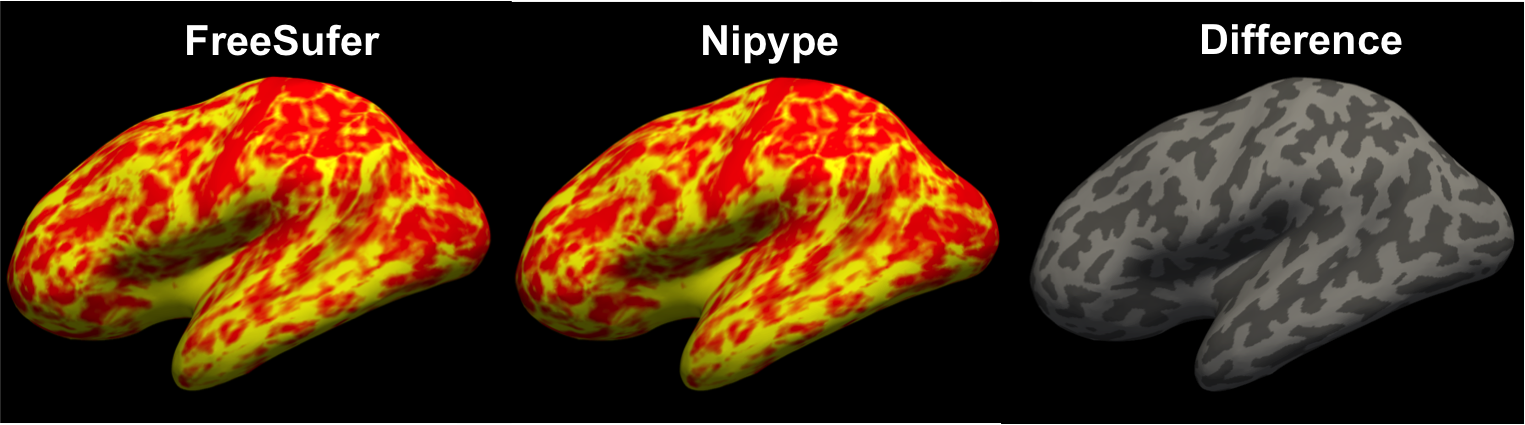
\includegraphics[width=.45\textwidth]{FS6NipypeDiff.png}
\caption{Visualization of the cortical thickness projected onto the left hemisphere's inflated surface for both the FreeSurfer(left) and \texttt{Nipype}(middle) workflows as well as the difference the two thicknesses(right). The thickness measurements showed no difference between the workflows.}
\end{figure}
%
%

\section{Conclusions}\label{conclusions}

The \texttt{Nipype} workflow created in this project was shown to be equivalent to the pre-existing FreeSurfer \texttt{recon-all} workflow.
Furthermore, by utilizing \texttt{Nipype}'s ability to run commands in parallel, the new workflow reduces the running time of \texttt{recon-all} by over 30\% when compared to FreeSurfer's \texttt{recon-all} script which runs commands in a sequential order. The \texttt{Nipype} environment also allows for increased collaboration in further developing the workflow.
Future work will involve incorporating more options to the \texttt{Nipype} workflow so that it can function as a complete replacement for the \texttt{tcsh} shell script.
The collaborations at the 2015 OHBM BrainHack meeting were instrumental in accomplishing this task.
Collaborations with the FreeSurfer, \texttt{Nipype}, and Human Connectome teams allowed members of this project to quickly identify problems and avoid unnecessary failures.

%%%%%%%%%%%%%%%%%%%%%%%%%%%%%%%%%%%%%%%%%%%%%%
%%                                          %%
%% Backmatter begins here                   %%
%%                                          %%
%%%%%%%%%%%%%%%%%%%%%%%%%%%%%%%%%%%%%%%%%%%%%%

\begin{backmatter}

\section*{Availability of Supporting Data}
The resulting workflow from this project can be found at: \url{\projURL}. An example of how to run the workflow on the \texttt{Nipype} tutorial data can be found at: \url{https://github.com/nipy/nipype/blob/master/examples/smri_fsreconall.py}.

\section*{Competing interests}
None

\section*{Author's contributions}
HJJ performed the project and wrote the report.
DGE created \texttt{Nipype} interfaces for the FreeSurfer commands, scripted the \texttt{Nipype} workflows, ran the workflow output comparisons, and contributed to the report. IO and RK advised on the project and contributed to the report.

\section*{Acknowledgements}
The authors would like to thank the organizers and attendees of the 2015 OHBM Hackathon.
This paper is funded by multiple grants: Huntington’s Disease Society of America (Human Biology Project Fellowship),   3D Shape Analysis for Computational Anatomy (R01 EB008171), Neurobiological Predictors of HD (R01 NS040068), Cognitive and Functional Brain Changes in Preclinical HD (R01 NS054893), Algorithms for Functional and Anatomical Brain Analysis (P41 RR015241), Enterprise Storage in a Collaborative Neuroimaging Environment (S10 RR023392), Core 2b HD (U54 EB005149), and Nipype (R03 EB008673).

%%%%%%%%%%%%%%%%%%%%%%%%%%%%%%%%%%%%%%%%%%%%%%%%%%%%%%%%%%%%%
%%                  The Bibliography                       %%
%%                                                         %%
%%  Bmc_mathpys.bst  will be used to                       %%
%%  create a .BBL file for submission.                     %%
%%  After submission of the .TEX file,                     %%
%%  you will be prompted to submit your .BBL file.         %%
%%                                                         %%
%%                                                         %%
%%  Note that the displayed Bibliography will not          %%
%%  necessarily be rendered by Latex exactly as specified  %%
%%  in the online Instructions for Authors.                %%
%%                                                         %%
%%%%%%%%%%%%%%%%%%%%%%%%%%%%%%%%%%%%%%%%%%%%%%%%%%%%%%%%%%%%%

% if your bibliography is in bibtex format, use those commands:
\bibliographystyle{bmc-mathphys} % Style BST file
\bibliography{brainhack-report} % Bibliography file (usually '*.bib' )

\end{backmatter}
\end{document}
